\section{Discussion}
Based on figures \ref{fig:regression-mehta} and 
\ref{fig:regression-mehta-article}, we see that the figure in article 
~\cite{HighBias} is similar to our own figures. 
Compared to the plots in the article our plots shows less noice, 
and some other small differences, but we see that the tendencies are the same.

\begin{figure}[H]
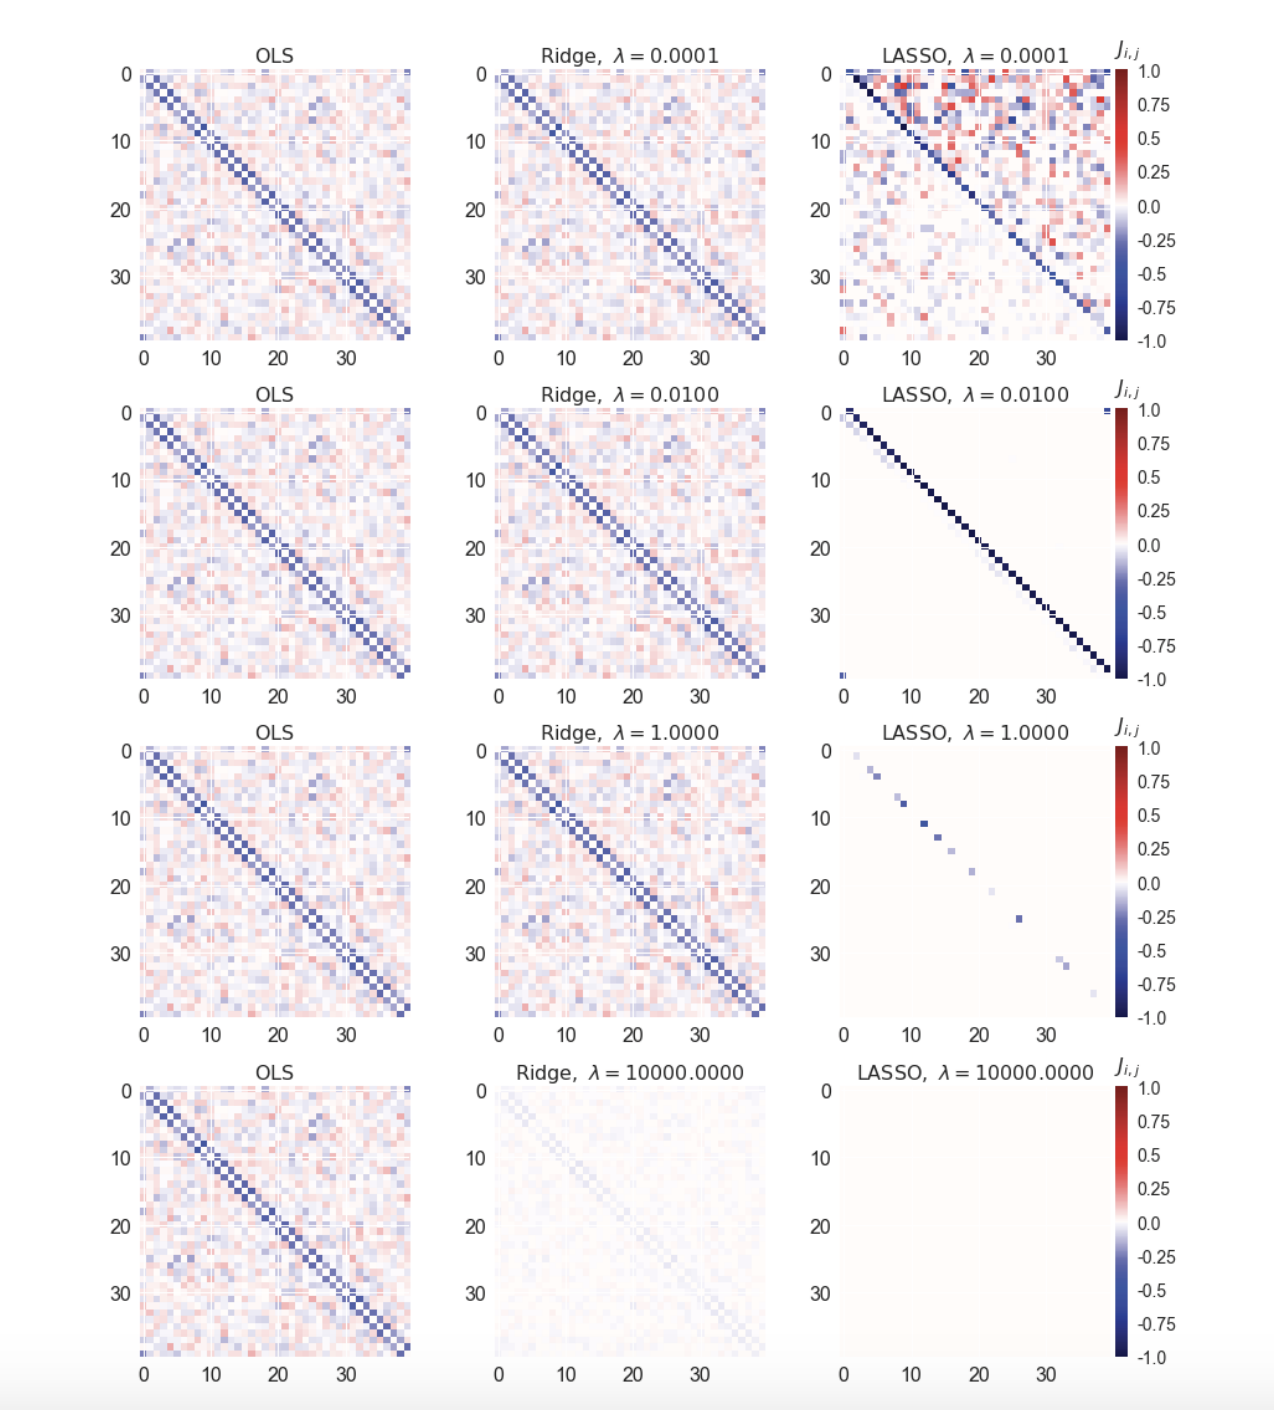
\includegraphics[width = 0.7\paperwidth]{figures/Regression_metha_article.png} 
\caption{Figures from article ~\cite{HighBias} shows similarities to the ones generated by our regression models.} 
\label{fig:regression-mehta-article}
\end{figure}

Looking at the R2 scores from figure \ref{fig:regression-r2}, we see 
that the R2 score for the training and test set follow each other closely. 
Again, comparing with articles plot, shown in figure 
\ref{fig:regression-r2-article}, we see the two have a similar shape 
but that there are a bigger diggerence between the R2 score for training 
data and the test data in the article. 
In the articles figure, the difference seems to be biggest for Ridge and 
OLS. As for our plot, it seems like Ridge has a bit bigger difference 
between the R2 score for training and test data than for the two other 
methods.

\begin{figure}[H]
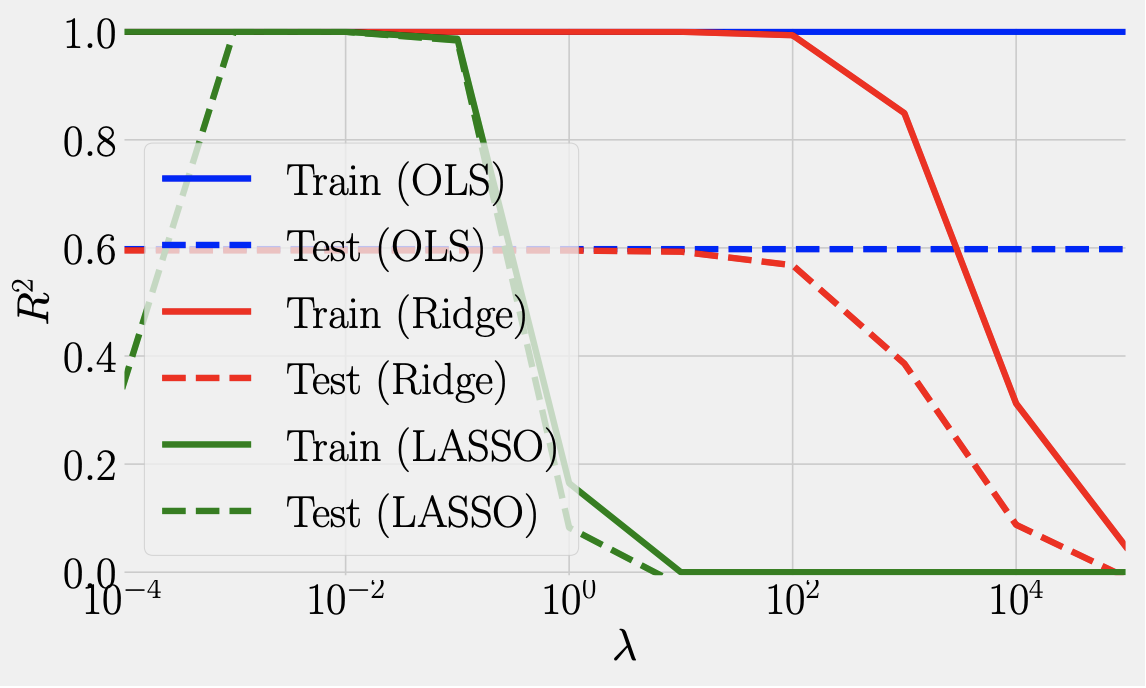
\includegraphics[width = 0.6\paperwidth]{figures/R2_article.png}
\caption{Performance of OLS, Ridge and LASSO regression on the Ising model as measured by the R2coefficient of determination.Figure 16 in ~\cite{HighBias}} 
\label{fig:regression-r2-article}
\end{figure}

To discuss the logistic regression model, 
we look at figure \ref{fig:logistic-eta}. For some $\eta$ the model 
quickly rises to an approximate highest value, but jumps back down to 
the equivalent of guessing from time
to time. When approaching 30 epochs and more, this behaviour 
seems to diminish somewhat, and overall the etas that produce 
the best results ($10^{-5} - 10^{-2}$) have most of their values
in the higher points.

Also table ~\ref{tab:logistic-critical} is connected 
to the logistic method model. We see that the accuracy is best
for \(\eta = 10^{-3}\). At its best, the accuracy is still 
way below one. 

Table ~\ref{tab:logistic-critical} can be compared to figure 
~\ref{fig:logistic-article}. We see that our model is slightly 
worse than the one described in the article, but that they 
follow the same tendencies. 

\begin{figure}[H]
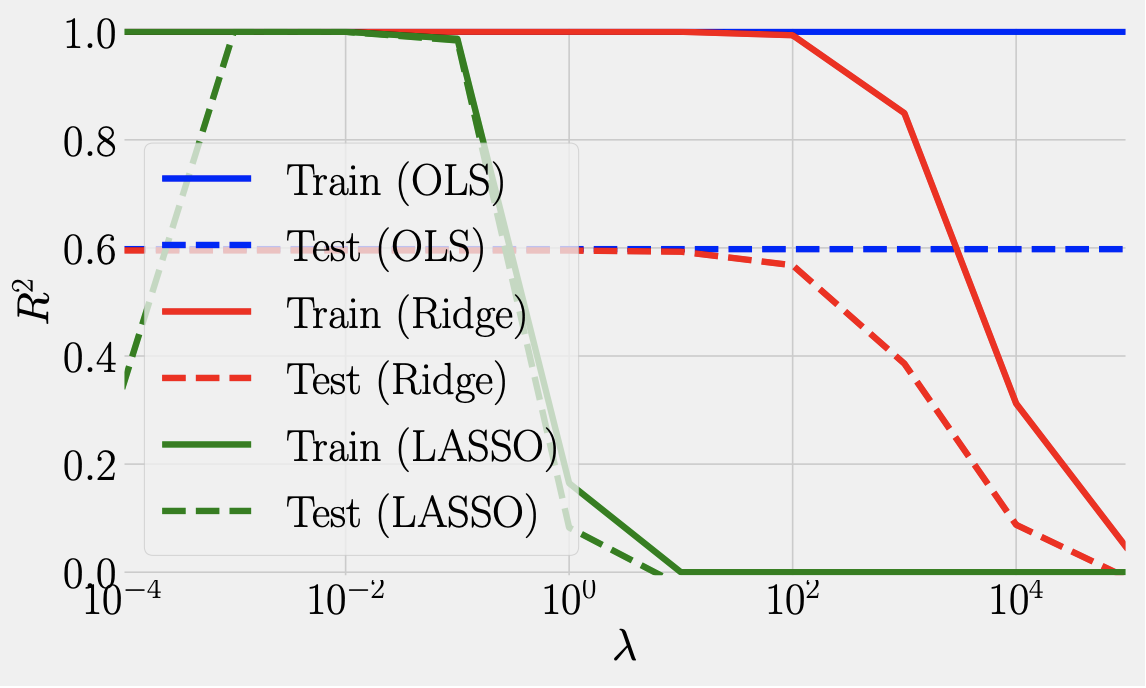
\includegraphics[width = 0.6\paperwidth]{figures/R2_article.png}
\caption{Accuracy as a function of the regularization parameter
\(\lambda\) in classifying the phases of the 2D Ising model on the
training (blue), test (red), and critical (green) data. The solid
and dashed lines compare the ’liblinear’ and ’SGD’ solvers, respectively..Figure 21 in ~\cite{HighBias}} 
\label{fig:logistic-article}
\end{figure}



